\section{The Models Language and Architecture}
% MS: This is a repeat of the content in the introduction

In the past Data Dictionaries were used to store details of database record structure or application data structure on a local per application basis, a metadata registry provides a similar capability but on a system or organisation-wide basis. It also provides features that are commonly included in a \emph{Thesaurus}, a \emph{Taxonomy}, and an \emph{Ontology} . These features include the ability to classify terms in relation to one another, record relationships such as synonyms, and classify hierarchical relationships. Ontologies have proved effective in matching what we have defined as the first problem, that is how domain concepts can be matched, however they are quite unwieldy to use when tackling the second problem of how to match and manage different representations.


Metadata Registries are normally found in Data Warehouses and Enterprise data mining systems, where vast quantities of data need to be administered and managed. It is likely that metadata registries will become more common as it becomes more and more necessary to deal with the recent internet-driven data explosion, especially as much of this data is unstructured, and can only be processed by relatively inefficient techniques.



This section takes key concepts from the ISO11179 standard and explores ways in which these concepts can be integrated with concepts and ideas embodied in model-driven engineering principles in order to design a metadata registry, which will both serve the practical purpose of allowing datasets to be matched, compared and managed, and allow for the development of a unified treatment of data in heterogeneous systems. The first part looks at the ISO standard and the ideas behind MOF, the second takes these ideas and uses them as the foundation for a specification of a metadata registry. The third section looks at how the metadata registry can be used to provide basic services for data-oriented model driven programming. In later chapters the practical and theoretical problems are examined in detailed to see in what ways full automated semantic interoperability can be achieved.


\subsection{ISO11179}
ISO11179 is the international standard relating to metadata and in particular metadata registries, and although there are a few other related standards which have informed the specification of the toolkit we describe ISO11179 provides the most exhaustive description of a metadata registry. It is therefore a key reference in this specification.




\begin{figure}[here]
	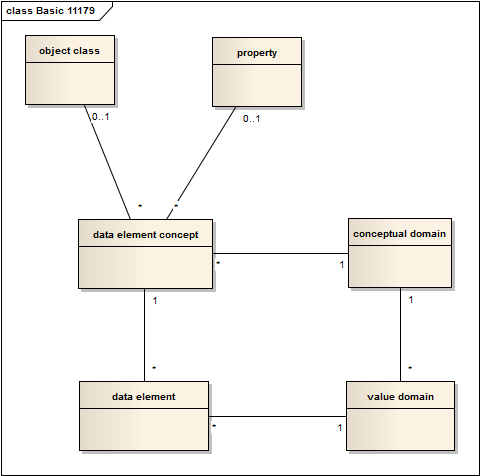
\includegraphics[width=0.48\textwidth,natwidth=610,natheight=642]{Basic11179}
	\caption{Core model for ISO11179 Metadata Registry} 
	\label{fig:basicMDR}
\end{figure}

The core ideas from the ISO11179 standard can be extracted to give us the notion of a \emph{data element concept}, \emph{a data element}, \emph{a value domain}, and a \emph{conceptual domain}. The standard currently confines itself to the detailed level of concepts and data elements and has no notion of collections of data elements or data element concepts, but instead attaches two attributes: an \emph{object class} and a \emph{property} to each DEC, these attributes allow DEC's to be aggregated or classified. This core model of the ISO11179 is illustrated in figure \ref{fig:basicMDR}.




\subsection{Metadata Registries - An Overview of Standards and Ideas}
%MS: This should be merged with the related work section.
\subsection{ISO11179}
ISO11179 is the international standard relating to metadata and in particular metadata registries, and although there are a few other related standards which I have examined in the course of specifying a metadata registry ISO11179 provides the most exhaustive description of a metadata registry. It is therefore a key reference in this specification. If we abstract the core ideas from the ISO11179 standard we have the notion of a \emph{data element concept}, \emph{a data element}, \emph{a value domain}, and a \emph{conceptual domain}. There is a four-way set of relationships between CDs, VDs, CDEs, and DECs which draws a distinctions between the conceptual or semantic \emph{level} and the representational \emph{level} in which these entities live, illustrated in figure\ref{fig:overviewMDR}.


\begin{figure}[here]
	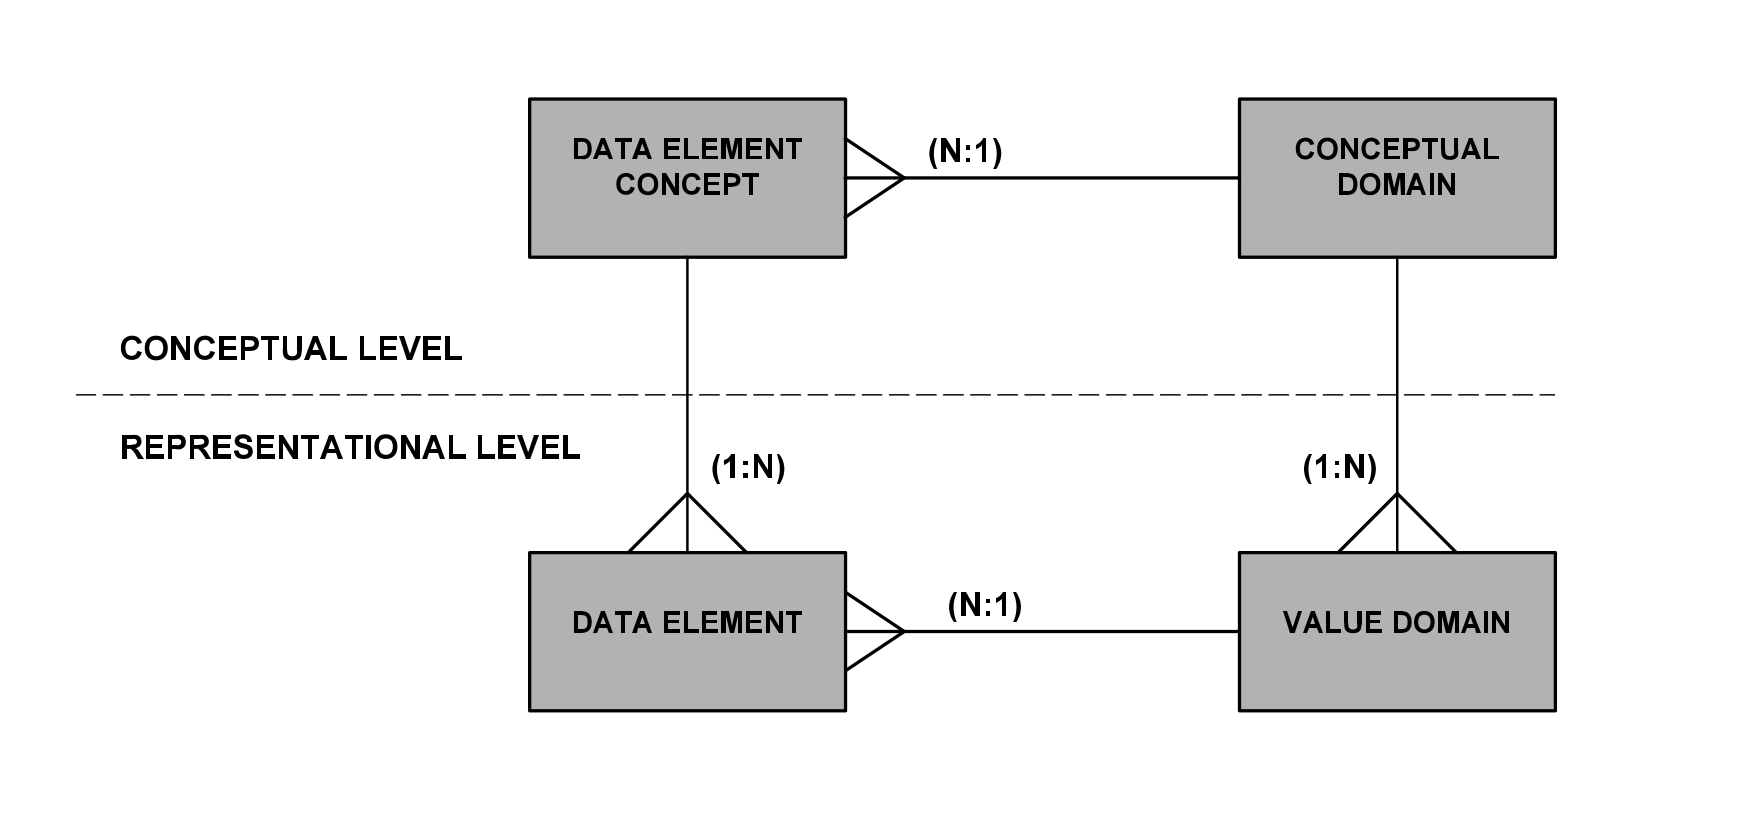
\includegraphics[width=0.5\textwidth,natwidth=610,natheight=642]{Overview11179}
	\caption{Overview model for a Metadata Registry} 
	\label{fig:overviewMDR}
\end{figure}

We can get some more hints as to the theory behind these guidelines in a related ISO standard \emph{ISO 20943-1: the standard for consistency in meta-data registries)} which states that the data element concept may relate several data elements that record data about that concept with different representations, implying that a single data element concept may have many value domains. It would appear therefore that what is intended is that a common data element in ISO11179 is really a relationship, or mapping between the set of data element concepts and the set of value domains. 

For example an Integer data-type in a programming language may be used to represent inches in a measurement program, it may also be used to count vehicles in a logistics application.  A data element is said to be comprised of a data element concept(DEC) which is its meaning and a value domain(VD) which is its representation.


\begin{table}[h]
	\begin{tabular}{ p{1.8cm} p{2.8cm}  p{3.0cm}  }  % centered columns (2 columns)
		\hline
		Entity & ISO Definition & ISO11179 Implementation Guidelines  \\ 
		\hline
		Data Element Concept(DEC) & An idea that can be represented in the form of a data element, described independently of any particular representation. & A concept that can be represented in the form of a Data Element, described independently of any particular representation.\\
		Common Data Element(CDE) & A unit of data for which the definition, identification, representation, and permissible values are specified by means of a set of attributes. & A unit of data for which the definition, identification, representation and Permissible Values are specified by means of a set of attributes. \\
		Value Domain (VD) & The description of a value meaning. & A description of a Value Meaning. \\
		Conceptual Domain (CD) & A set of valid value meanings, which may be enumerated or expressed via a description.& A set of valid Value Meanings.\\
		\hline
	\end{tabular}
\end{table}

\vspace{5.mm}


The simple mapping between DEC's and VD's is perhaps better replaced with a functional relationship, and in section 2 we will explore the idea of a functional relationship between the two, its advantages and disadvantages. For now we will just try and describe the MDR according to the ISO specification. If we consider a single model of a system then we are putting constraints on the extent of the VD's, or if a set of VD's is considered to be a conceptual domain then we are constraining the model to a single CD.  By doing this we can model the system using functional relationships, so make a total function relating the model DEC's to the VD's \emph{in a particular conceptual domain}, since all the DEC's will have a mapping to a VD. It is not an injective function because of course more than one DEC can use the same representation or VD, and it is not surjective because there can be VD's in that particular Conceptual Domain which are not used in the model. It may be that a more useful model can be built by using the term Conceptual Domain to mean just those elements related to a \emph{group} of data elements, in which case we could specify a surjective relationship.  The ISO standard does not specify anything about \emph{groups} of data elements, so it would be perfectly reasonable to introduce just such a constraint. 


As an illustration lets take the case of a medical systems model in which there may be some data elements, let's say \emph{blood pressure} and \emph{location}, which are being recorded.  However it may not be, in which case no actual values of depth will be recorded, measured or used in the system. In the implementation we are using the set of value domains mapped to actual values (VAL), and so the blood pressure (BP) can be viewed as a partial function, since there may be data points taken at times when other values are measured and not the blood pressure:
\begin{zed}
	[VAL]\\
	BP == VD \pfun VAL
\end{zed}
 
 

Consider the definition of a \emph{Conceptual Domain}:
\begin{quote}
	A conceptual domain is a set of value meanings. The intention of a conceptual domain is to detail the model's value meanings. Many value domains may be in the extension of the same conceptual domain, but a value domain is associated with one conceptual domain. Conceptual domains may have relationships with other conceptual domains, so it is possible to create a concept system of conceptual domains. Value domains may have relationships with other value domains, which provide the framework to capture the structure of sets of related value domains and their associated concepts.	
\end{quote}
Conceptual domains comprise sets of value domains, however in the current prototype implementation of conceptual Domains has been omitted, since there has been up to now no use case warranting their inclusion.

\subsection{A Metadata Language and Abstract Architecture }

The ISO11179 specification illustrates different aspects of the standard using UML class diagrams, we have used these to inform the development of a very simple domain specific language, which we are calling \textbf{DataMOF} based on the standard. The main differences are that we have added in containers to handle data element collections, calling these \emph{Classes} and to handle collections of these \emph{Classes} which we have called \emph{Models}.

A simplified overview model, without attributes and methods, showing the Ecore model for the DataMOF DSL is shown in Figure \ref{fig:mcSimplifiedOverview}.

\begin{figure}[here]
	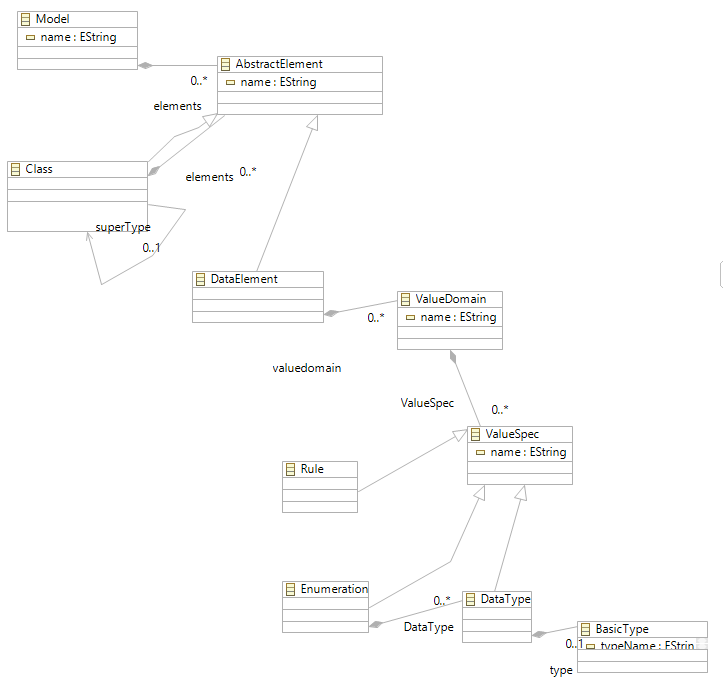
\includegraphics[width=0.5\textwidth,natwidth=610,natheight=642]{DMOF_EcoreDiagram}
	\caption{Overview Ecore DSL for Model Catalogue} 
	\label{fig:mcSimplifiedOverview}
\end{figure}

\subsubsection{Model}
A model is a grouping or containment entity which groups a set of \emph{Classes} together. Models can be thought of as datasets, or even database schemas, very often in the medical domain they are defined either by XML Schema definition files, or by equivalent schemas written in Excel. 
Models are collections of either \emph{Data Elements} or \emph{Classes}. This aspect is captured in the \emph{Emfatic} representation by the \emph{AbstractElement} which can be either a  \emph{Data Element} or a \emph{Class}  There is no real notion of composition or multiplicity, a instance of a Model can contain an instance of a Data Element or not as required by the instance.  Models are named, have a description and have a version identity.
\subsubsection{Class}
A Class is a grouping or collection of \emph{attributes} which can be data elements or classes, the attributes are currently \emph{mandatory}, so that class with 5 attributes must have those 5 attributes instantiated in an instance for it to be considered of that class. Classes represent \emph{Concepts}, (***This is not true present****)and can be \emph{Generalized} into a hierarchy(**but we might get it implemented before the paper comes out**). The idea of a \emph{Data Element Concept} was omitted from the initial prototype, although it has been added to later versions of the language.
\subsection{Data Elements} 
Data Elements can also represent \emph{Concepts} and are by their nature \emph{atomic}.  Each data element is related to a value domain on a one-to-one basis, and the relationship is a two-way relationship.
\subsection{Value Domain}
A Value Domain is the domain in which the data element is represented, it can consist of one or more \emph{ValueSpecs}.
\subsection{ValueSpec}
A \emph{ValueSpec} can be a simple datatype, an enumeration of datatypes, or a rule - such as a regular expression - which defines the way in which a series of characters is formed into a string attribute. 




\lstinputlisting[label=DMof,caption=DMOF in Emfatic Notation]{ASEFigs/DataMOF.emf}


 




